\documentclass[]{article}
\usepackage{lmodern}
\usepackage{amssymb,amsmath}
\usepackage{ifxetex,ifluatex}
\usepackage{fixltx2e} % provides \textsubscript
\ifnum 0\ifxetex 1\fi\ifluatex 1\fi=0 % if pdftex
  \usepackage[T1]{fontenc}
  \usepackage[utf8]{inputenc}
\else % if luatex or xelatex
  \ifxetex
    \usepackage{mathspec}
  \else
    \usepackage{fontspec}
  \fi
  \defaultfontfeatures{Ligatures=TeX,Scale=MatchLowercase}
\fi
% use upquote if available, for straight quotes in verbatim environments
\IfFileExists{upquote.sty}{\usepackage{upquote}}{}
% use microtype if available
\IfFileExists{microtype.sty}{%
\usepackage{microtype}
\UseMicrotypeSet[protrusion]{basicmath} % disable protrusion for tt fonts
}{}
\usepackage[margin=1in]{geometry}
\usepackage{hyperref}
\hypersetup{unicode=true,
            pdftitle={Exploring water quality},
            pdfauthor={Nicolas F. S-Gelais},
            pdfborder={0 0 0},
            breaklinks=true}
\urlstyle{same}  % don't use monospace font for urls
\usepackage{color}
\usepackage{fancyvrb}
\newcommand{\VerbBar}{|}
\newcommand{\VERB}{\Verb[commandchars=\\\{\}]}
\DefineVerbatimEnvironment{Highlighting}{Verbatim}{commandchars=\\\{\}}
% Add ',fontsize=\small' for more characters per line
\usepackage{framed}
\definecolor{shadecolor}{RGB}{248,248,248}
\newenvironment{Shaded}{\begin{snugshade}}{\end{snugshade}}
\newcommand{\KeywordTok}[1]{\textcolor[rgb]{0.13,0.29,0.53}{\textbf{#1}}}
\newcommand{\DataTypeTok}[1]{\textcolor[rgb]{0.13,0.29,0.53}{#1}}
\newcommand{\DecValTok}[1]{\textcolor[rgb]{0.00,0.00,0.81}{#1}}
\newcommand{\BaseNTok}[1]{\textcolor[rgb]{0.00,0.00,0.81}{#1}}
\newcommand{\FloatTok}[1]{\textcolor[rgb]{0.00,0.00,0.81}{#1}}
\newcommand{\ConstantTok}[1]{\textcolor[rgb]{0.00,0.00,0.00}{#1}}
\newcommand{\CharTok}[1]{\textcolor[rgb]{0.31,0.60,0.02}{#1}}
\newcommand{\SpecialCharTok}[1]{\textcolor[rgb]{0.00,0.00,0.00}{#1}}
\newcommand{\StringTok}[1]{\textcolor[rgb]{0.31,0.60,0.02}{#1}}
\newcommand{\VerbatimStringTok}[1]{\textcolor[rgb]{0.31,0.60,0.02}{#1}}
\newcommand{\SpecialStringTok}[1]{\textcolor[rgb]{0.31,0.60,0.02}{#1}}
\newcommand{\ImportTok}[1]{#1}
\newcommand{\CommentTok}[1]{\textcolor[rgb]{0.56,0.35,0.01}{\textit{#1}}}
\newcommand{\DocumentationTok}[1]{\textcolor[rgb]{0.56,0.35,0.01}{\textbf{\textit{#1}}}}
\newcommand{\AnnotationTok}[1]{\textcolor[rgb]{0.56,0.35,0.01}{\textbf{\textit{#1}}}}
\newcommand{\CommentVarTok}[1]{\textcolor[rgb]{0.56,0.35,0.01}{\textbf{\textit{#1}}}}
\newcommand{\OtherTok}[1]{\textcolor[rgb]{0.56,0.35,0.01}{#1}}
\newcommand{\FunctionTok}[1]{\textcolor[rgb]{0.00,0.00,0.00}{#1}}
\newcommand{\VariableTok}[1]{\textcolor[rgb]{0.00,0.00,0.00}{#1}}
\newcommand{\ControlFlowTok}[1]{\textcolor[rgb]{0.13,0.29,0.53}{\textbf{#1}}}
\newcommand{\OperatorTok}[1]{\textcolor[rgb]{0.81,0.36,0.00}{\textbf{#1}}}
\newcommand{\BuiltInTok}[1]{#1}
\newcommand{\ExtensionTok}[1]{#1}
\newcommand{\PreprocessorTok}[1]{\textcolor[rgb]{0.56,0.35,0.01}{\textit{#1}}}
\newcommand{\AttributeTok}[1]{\textcolor[rgb]{0.77,0.63,0.00}{#1}}
\newcommand{\RegionMarkerTok}[1]{#1}
\newcommand{\InformationTok}[1]{\textcolor[rgb]{0.56,0.35,0.01}{\textbf{\textit{#1}}}}
\newcommand{\WarningTok}[1]{\textcolor[rgb]{0.56,0.35,0.01}{\textbf{\textit{#1}}}}
\newcommand{\AlertTok}[1]{\textcolor[rgb]{0.94,0.16,0.16}{#1}}
\newcommand{\ErrorTok}[1]{\textcolor[rgb]{0.64,0.00,0.00}{\textbf{#1}}}
\newcommand{\NormalTok}[1]{#1}
\usepackage{graphicx,grffile}
\makeatletter
\def\maxwidth{\ifdim\Gin@nat@width>\linewidth\linewidth\else\Gin@nat@width\fi}
\def\maxheight{\ifdim\Gin@nat@height>\textheight\textheight\else\Gin@nat@height\fi}
\makeatother
% Scale images if necessary, so that they will not overflow the page
% margins by default, and it is still possible to overwrite the defaults
% using explicit options in \includegraphics[width, height, ...]{}
\setkeys{Gin}{width=\maxwidth,height=\maxheight,keepaspectratio}
\IfFileExists{parskip.sty}{%
\usepackage{parskip}
}{% else
\setlength{\parindent}{0pt}
\setlength{\parskip}{6pt plus 2pt minus 1pt}
}
\setlength{\emergencystretch}{3em}  % prevent overfull lines
\providecommand{\tightlist}{%
  \setlength{\itemsep}{0pt}\setlength{\parskip}{0pt}}
\setcounter{secnumdepth}{0}
% Redefines (sub)paragraphs to behave more like sections
\ifx\paragraph\undefined\else
\let\oldparagraph\paragraph
\renewcommand{\paragraph}[1]{\oldparagraph{#1}\mbox{}}
\fi
\ifx\subparagraph\undefined\else
\let\oldsubparagraph\subparagraph
\renewcommand{\subparagraph}[1]{\oldsubparagraph{#1}\mbox{}}
\fi

%%% Use protect on footnotes to avoid problems with footnotes in titles
\let\rmarkdownfootnote\footnote%
\def\footnote{\protect\rmarkdownfootnote}

%%% Change title format to be more compact
\usepackage{titling}

% Create subtitle command for use in maketitle
\newcommand{\subtitle}[1]{
  \posttitle{
    \begin{center}\large#1\end{center}
    }
}

\setlength{\droptitle}{-2em}
  \title{Exploring water quality}
  \pretitle{\vspace{\droptitle}\centering\huge}
  \posttitle{\par}
  \author{Nicolas F. S-Gelais}
  \preauthor{\centering\large\emph}
  \postauthor{\par}
  \predate{\centering\large\emph}
  \postdate{\par}
  \date{2018-05-08}

\usepackage{booktabs}
\usepackage{longtable}
\usepackage{array}
\usepackage{multirow}
\usepackage[table]{xcolor}
\usepackage{wrapfig}
\usepackage{float}
\usepackage{colortbl}
\usepackage{pdflscape}
\usepackage{tabu}
\usepackage{threeparttable}
\usepackage[normalem]{ulem}

\begin{document}
\maketitle

\subsubsection{Read files}\label{read-files}

Import the canadian rivers dataset data on stations and the canadian
guidelines

\begin{Shaded}
\begin{Highlighting}[]
\KeywordTok{library}\NormalTok{(knitr)}
\KeywordTok{library}\NormalTok{(kableExtra)}
\KeywordTok{library}\NormalTok{(ReporteRs)}
\KeywordTok{library}\NormalTok{(maps)}
\KeywordTok{library}\NormalTok{(fmsb)}
\KeywordTok{library}\NormalTok{(dplyr)}
\KeywordTok{library}\NormalTok{(ggplot2)}
\KeywordTok{library}\NormalTok{(tidyr)}
\KeywordTok{rm}\NormalTok{(}\DataTypeTok{list=}\KeywordTok{ls}\NormalTok{(}\DataTypeTok{all=}\OtherTok{TRUE}\NormalTok{))}
\KeywordTok{source}\NormalTok{(}\StringTok{"R/functions.R"}\NormalTok{)}
\KeywordTok{load}\NormalTok{(}\StringTok{"data/dataCDN.RData"}\NormalTok{)}
\KeywordTok{load}\NormalTok{(}\StringTok{"data/sitesClassfc.RData"}\NormalTok{)}
\KeywordTok{load}\NormalTok{(}\StringTok{"data/critLimdoc.RData"}\NormalTok{)}
\NormalTok{colFreq<-}\ControlFlowTok{function}\NormalTok{(x)}\KeywordTok{sum}\NormalTok{(}\OperatorTok{!}\KeywordTok{is.na}\NormalTok{(x))}\OperatorTok{/}\KeywordTok{length}\NormalTok{(x)}
\end{Highlighting}
\end{Shaded}

\subsubsection{1. Compare ecoservices
guidelines}\label{compare-ecoservices-guidelines}

We created a common database with all the Canadian guidelines for the
selected ecosystes services and for trohpic status guidelines we used
Dodd 19XX trophic status classification. A total of 178 variables are
used to establish these guidelines. To assess the amount of overlap
between the guidelines used, we grouped the guidelines by chemical
groups (based on the CCME classifiation) and calculated the proportion
of guidelines from each chemical group that is used for a specific ES
(See Table 1). For each chemical group we selected variables that had
the most impotant overlap between the different ES and searched for
those variables within a variety of canadian openly available databases.

For irrigation and livestock, most guidelines are for pesticides and
metals, while for drinking and aquatic wildlife, most guidelines are for
pesticides and organic chemicals. For recreational activities guidelines
are biollogical, physical and ph, while for trophic state guidelines are
mostly for inorganic chemicals (i.e.~nutrients).

Table 1: The proportion of guidelines in each chemical group by
ecosystem services (ES) based on Canadian guidelines and

ES

Biological

Inorganic chemicals

Metals

Nutrients

Organic chemicals

Pesticides

Aquatic Wildlife

{0}

{0.06}

{0.15}

{0}

{0.47}

{0.29}

Drinking

{0.07}

{0.08}

{0.14}

{0}

{0.26}

{0.34}

Irrigation

{0.06}

{0.03}

{0.41}

{0}

{0.06}

{0.44}

Livestock

{0}

{0.06}

{0.25}

{0}

{0.22}

{0.46}

Recreational

{0.33}

{0}

{0}

{0}

{0}

{0}

Trophic Status

{0.2}

{0}

{0}

{0.8}

{0}

{0}

\begin{center}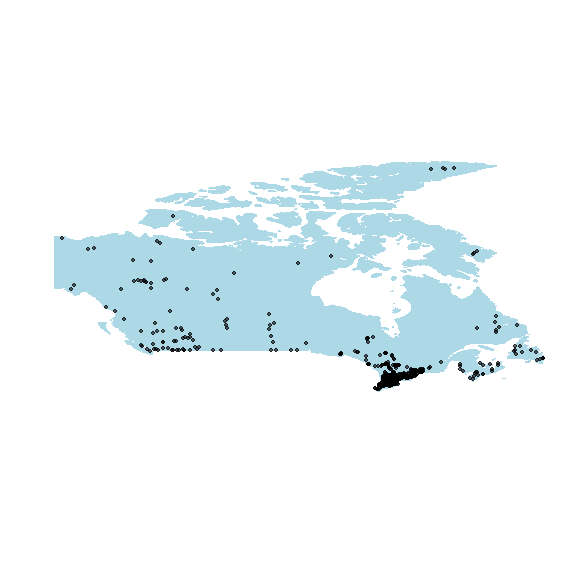
\includegraphics{figures/map -1} \end{center}

\begin{verbatim}
## pdf 
##   2
\end{verbatim}

\begin{verbatim}
## [1] 0.08627159
\end{verbatim}

\begin{table}[H]
\centering
\begin{tabular}{l|l|l|l|l|l|l|l|l|l|l|l|l|l|l|l|l|l|l|l|l|l|l}
\hline
\multicolumn{ 1}{c|}{ } & \multicolumn{11}{|c|}{Group 1} & \multicolumn{11}{|c}{Group 2} \\
\cline{2-12} \cline{13-23}
\rotatebox{45}{ } & \rotatebox{45}{fc} & \rotatebox{45}{chloride} & \rotatebox{45}{fluoride} & \rotatebox{45}{nitrate} & \rotatebox{45}{nitrite} & \rotatebox{45}{arsenic} & \rotatebox{45}{cadmium} & \rotatebox{45}{copper} & \rotatebox{45}{iron} & \rotatebox{45}{lead} & \rotatebox{45}{molybdenum} & \rotatebox{45}{nickel} & \rotatebox{45}{uranium} & \rotatebox{45}{zinc} & \rotatebox{45}{tn} & \rotatebox{45}{tp} & \rotatebox{45}{toluene} & \rotatebox{45}{atrazine} & \rotatebox{45}{bromoxynil} & \rotatebox{45}{dicamba} & \rotatebox{45}{metolachlor} & \rotatebox{45}{simazine}\\
\hline
Chemical.groups & Biological & Inorganic chemical & Inorganic chemical & Inorganic chemical & Inorganic chemical & Metal & Metal & Metal & Metal & Metal & Metal & Metal & Metal & Metal & Nutrients & Nutrients & Organic chemical & Pesticide & Pesticide & Pesticide & Pesticide & Pesticide\\
\hline
aquatic &  & 120000 & 120 & 13000 & 11820 & 5 & 0.09 & 2 & 300 & 1 & 73 & 25 & 15 & 30 &  &  & 2 & 1.8 & 5 & 10 & 7.8 & 10\\
\hline
drink & 11 &  & 1500 & 45000 & 3000 & 10 & 5 &  &  & 10 &  &  & 20 &  &  &  & 60 & 5 & 5 & 120 & 50 & 10\\
\hline
irrigation & 100 &  & 1000 &  &  & 100 & 5.1 &  & 5000 & 200 &  & 200 & 10 &  &  &  &  & 10 & 0.33 & 0.006 & 28 & 0.5\\
\hline
livestock &  &  &  &  & 10000 & 25 & 80 &  &  & 100 & 500 & 1000 & 200 & 50000 &  &  & 24 & 5 & 11 & 122 & 50 & 10\\
\hline
mesotrophic &  &  &  &  &  &  &  &  &  &  &  &  &  &  & 1500 & 75 &  &  &  &  &  & \\
\hline
oligotrophic &  &  &  &  &  &  &  &  &  &  &  &  &  &  & 700 & 25 &  &  &  &  &  & \\
\hline
recreational & 200 &  &  &  &  &  &  &  &  &  &  &  &  &  &  &  &  &  &  &  &  & \\
\hline
freq & 8.63 & 76.78 & 15.51 & 73.65 & 80.73 & 23.99 & 60.02 & 75.98 & 77.20 & 48.54 & 59.11 & 62.00 & 25.82 & 75.33 & 28.42 & 96.10 & 0.36 & 0.01 & 0.00 & 0.00 & 0.12 & 0.11\\
\hline
\end{tabular}
\end{table}

\subsubsection{2.Compare ecoservices in the
dataset}\label{compare-ecoservices-in-the-dataset}

In this table, we compare the occurence of the different ecoservices in
the dataset. On the diagonal of this table, the proportion of sites for
which a given criteria was met is reported. Outside the diagonal we are
reporting how often the column criteria is met when the row criteria is
met.

oligotrophic

mesotrophic

eutrophic

aquatic

recreational

drink

irrigation

livestock

oligotrophic

0.32

0.00

0.00

0.29

0.85

0.25

0.71

1

mesotrophic

0.00

0.39

0.00

0.20

0.69

0.14

0.52

1

eutrophic

0.00

0.00

0.18

0.09

0.31

0.05

0.22

1

aquatic

0.44

0.37

0.08

0.22

0.81

0.22

0.66

1

recreational

0.41

0.40

0.08

0.26

0.66

0.23

0.78

1

drink

0.52

0.36

0.05

0.30

1.00

0.15

1.00

1

irrigation

0.44

0.39

0.07

0.27

1.00

0.30

0.51

1

livestock

0.33

0.39

0.18

0.22

0.67

0.16

0.52

1

In this dataset, 32 \% of sites were oligotrophic, 39 \% mesotrophic and
18\% eutrophic. Only 22\% of the samples were suitable for aquatic life,
66\% for swimming and 15\% for drinking. For gricultural use, in 51\% of
the samples the water was usable for irrigation and 100\% for livestock.

When the water is oligotrophic are more often suitable for aquatic life
(29\%), recreation (85\%), drinking (25\%) and irrigation (71\%) than
mesotrpohic and eutrophic samples.

Because, the drinking and livestock criteria were met in the vast
majority of samples, they were not included in the analyses.

\begin{verbatim}
##        [,1]
## red   0.116
## green 0.828
## blue  0.116
\end{verbatim}

\begin{center}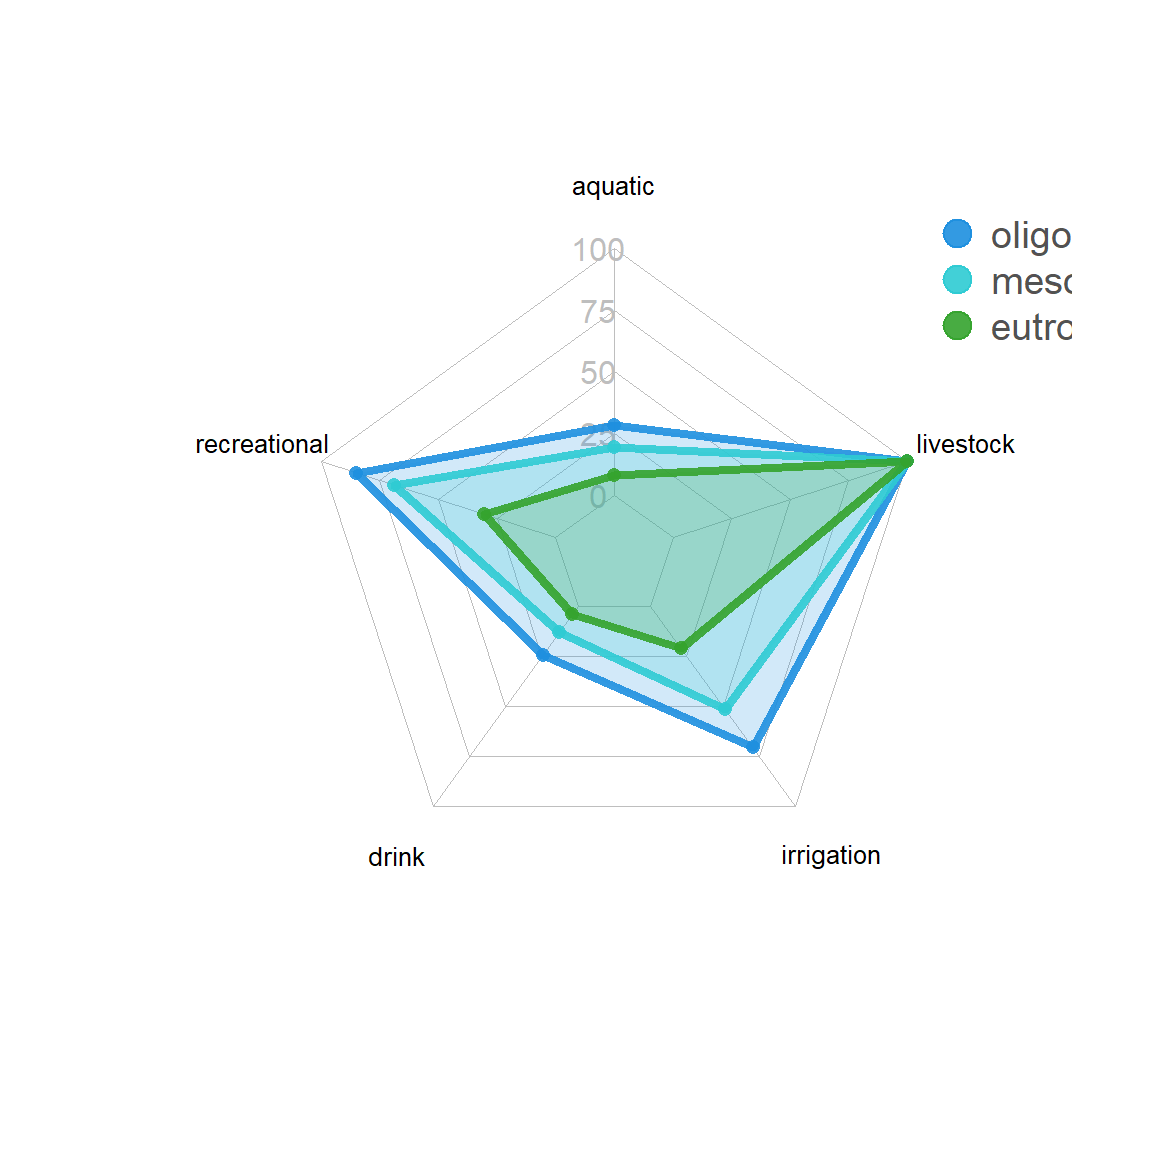
\includegraphics{figures/radar plot  -1} \end{center}

\begin{center}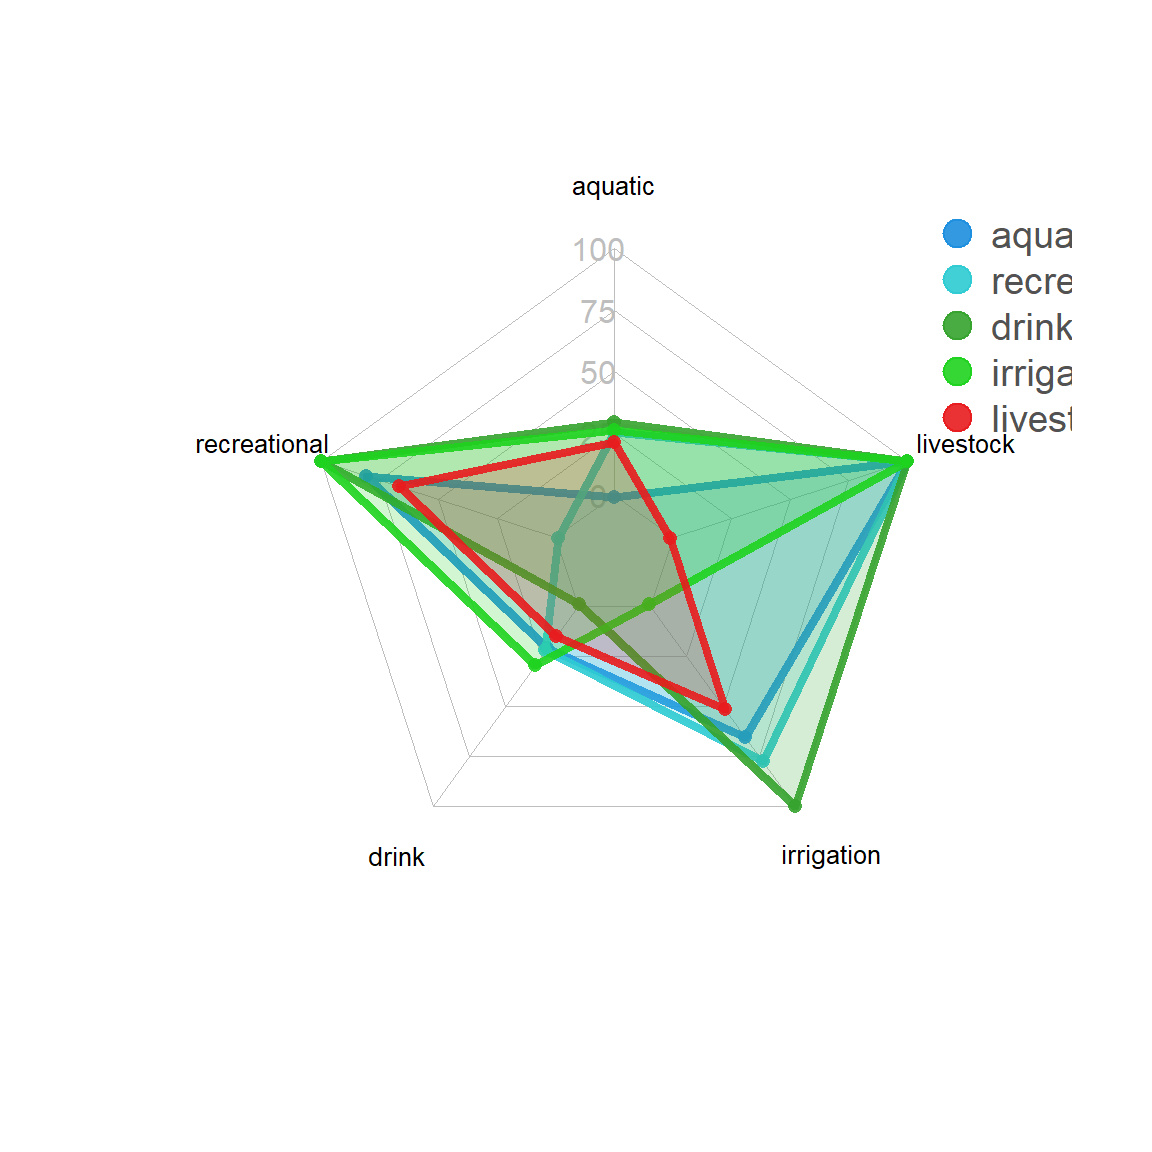
\includegraphics{figures/radar plot  -2} \end{center}

\paragraph{Ecoservices PCA}\label{ecoservices-pca}

\begin{center}\rule{0.5\linewidth}{\linethickness}\end{center}

In the ecoservices PCA, the first and second axes are mainly trophic
axes, on which, all ecoservices are more associated with oligotrophic
water. On the third axis, we see a strong association between
recreational and irrgations services, and between aquatic wildlife and
drinking, but a negative association between the two groups. By looking
at the ecoservices guideline table, it make sense that aquatic wildlife
and drinking are associated, as their respectives guidelines are
similar, but it isn't the case for irrigation and recreation.

\begin{center}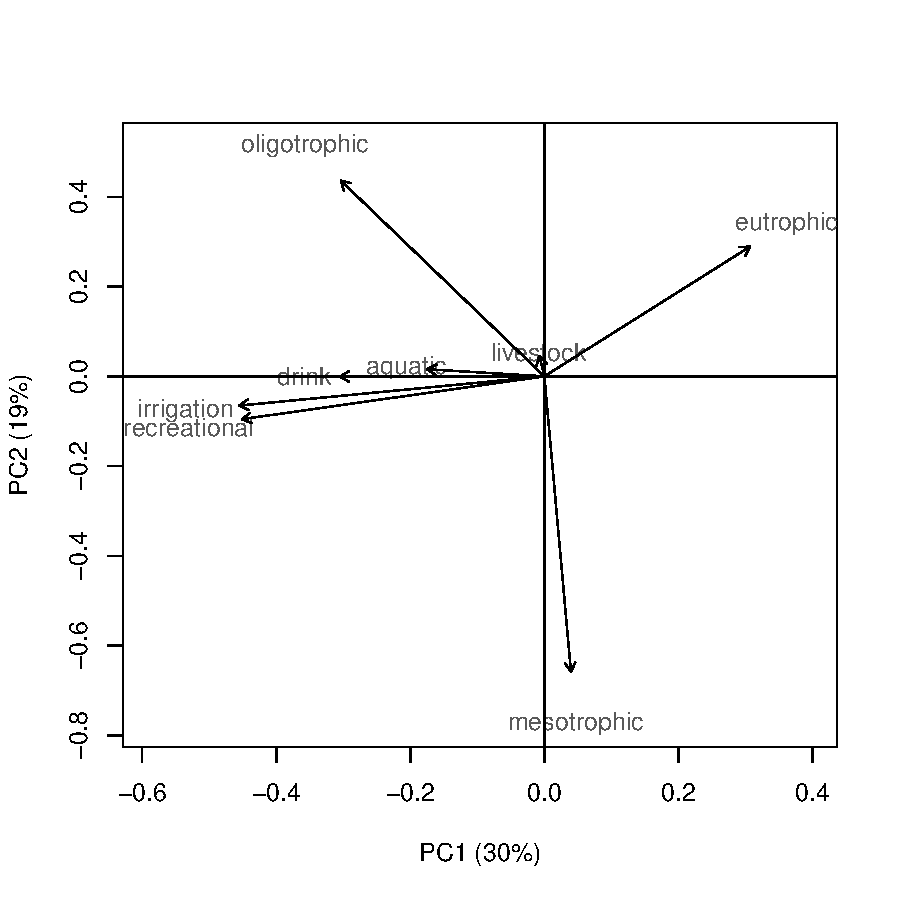
\includegraphics{figures/services PCA-1} \end{center}

\begin{center}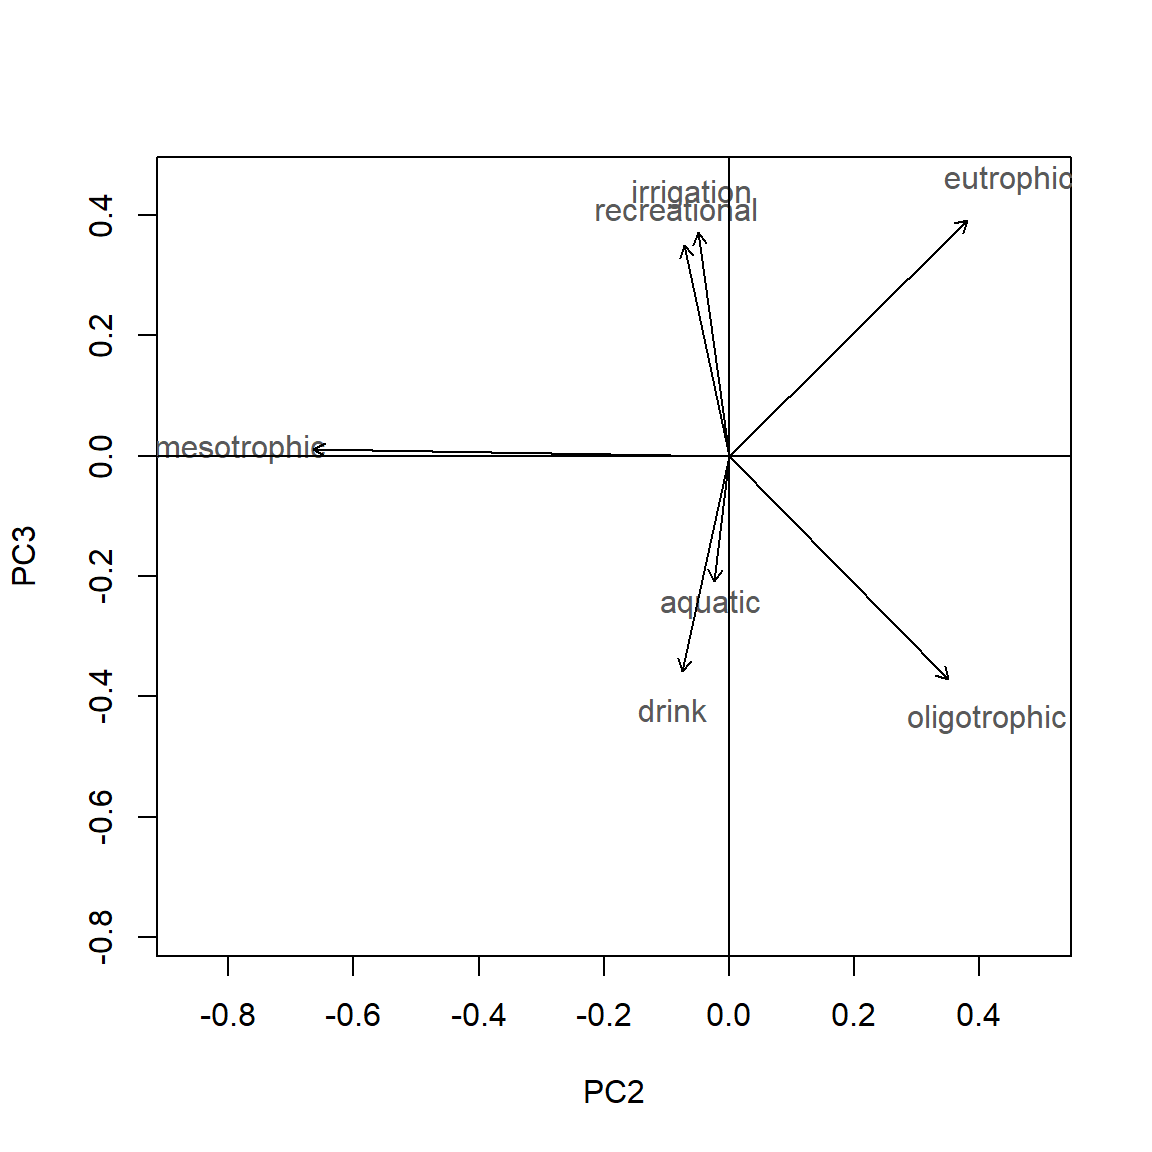
\includegraphics{figures/services PCA-2} \end{center}

\paragraph{Comparing the limiting
guidelines}\label{comparing-the-limiting-guidelines}

\begin{center}\rule{0.5\linewidth}{\linethickness}\end{center}

In this table we compare the limiting guidelines for each ecoservice.
For each guideline, we report how often when a sample cannot provide an
ecoservice a specific guideline responsible for the none compliance. For
trophic status, when a sample change from one trophic status to the
other, TN and TP are almost always both over the guideline (Even if TP
was measure more often)


\end{document}
